\begin{frame}{Open games}
	\textbf{Warning}: Open games are compositional structures, hence the single building blocks do not make much sense from a classical standpoint -- you have to put them together to get something meaningful!

	\vfill
	Intuitively, an 'atomic' open game is a forest of bushes:

	\begin{center}
		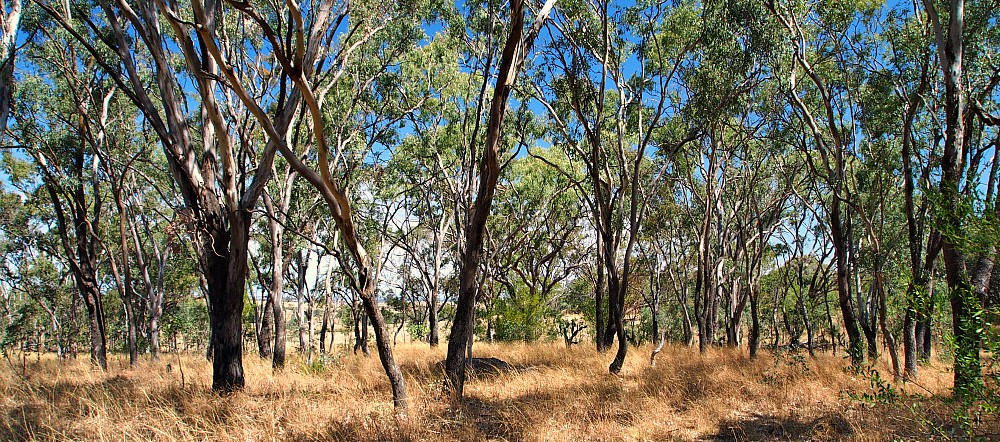
\includegraphics[width=.9\textwidth]{figures/bush_forest.jpg}
	\end{center}
\end{frame}

\begin{frame}{Back and forth}
	\vspace{-5ex}
	\begin{center}
		\hspace{10ex}
		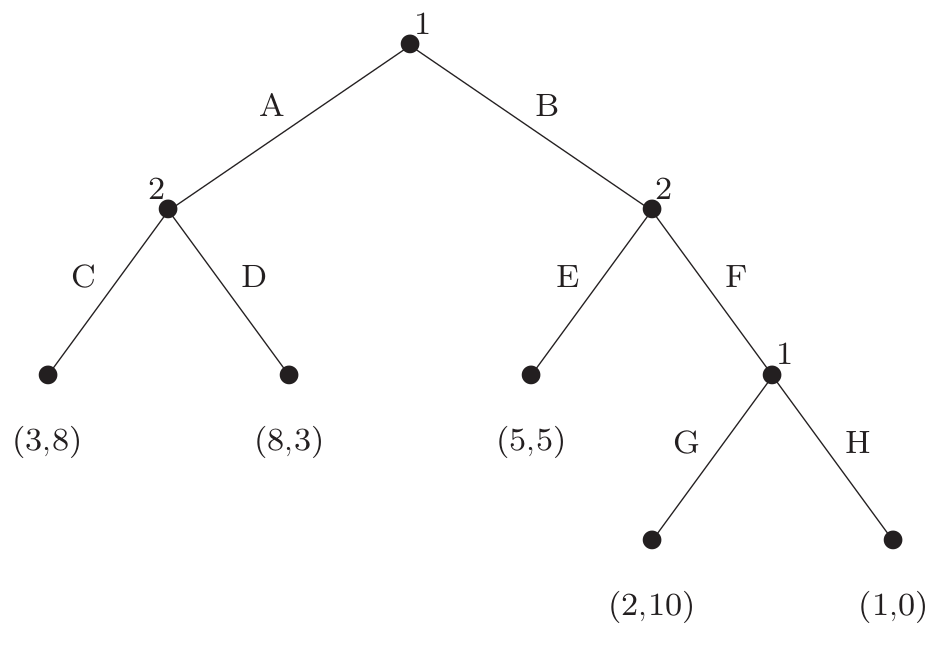
\includegraphics[width=.5\textwidth]{figures/ext_game.png}
	\end{center}

	\vspace{-6ex}
	There's two phases in a game*
	\begin{enumerate}
		\item The `\textbf{forward phase}'\\
		Players take turns and make their own decisions until a leaf is reached
		\item The `\textbf{backward phase}'\\
		Payoffs propagate back to players along the tree\\
		\qquad $\longto$ \textbf{backward induction}
	\end{enumerate}

	\vfill
	{\color{colornote}*handwaving important philosophical point here}
\end{frame}

\begin{frame}{Lenses and bidirectional information flows}
	A \textbf{lens} models exactly this bidirectional information flow:

	\begin{center}
		\includegraphics[clip, page=1, trim=1cm 10cm 1cm 5.6cm, width=.75\textwidth]{figures/drawings.pdf}
	\end{center}

	\vspace{-2ex}
	\begin{definition}
		Let $\cat C$ be a cartesian category {\color{colornote}(think: sets \& functions)}.\\
		A \textbf{lens} $(X,S) \to (Y,R)$ is a pair of maps
		\begin{equation*}
			\mathsf{view} : X \to Y, \qquad
			\mathsf{update} : X \times R \to S
		\end{equation*}
	\end{definition}

	\vspace{-2ex}
	{\color{colornote}They can be generalized greatly, see \textbf{optics} \cite{riley2018optics}}
\end{frame}

\begin{frame}{Games as lenses}
	A game can be represented naively as a lens

	\begin{center}
		\includegraphics[clip, page=2, trim=4cm 8cm 4cm 5.6cm, width=\textwidth]{figures/drawings.pdf}
	\end{center}
\end{frame}

\begin{frame}{What's coutility?}

	\vfill
	\begin{quotation}
		For a given node $x$ in a game, a player’s continuation value (also called \textbf{continuation payoff}) is the payoff that this \textbf{player will eventually get} contingent on the path of play \textbf{passing through node $x$}.
		{\color{colornote}-- Strategy \cite{watson2002strategy}}
	\end{quotation}

	\vfill
	The coplay function takes on this job. In classical game theory it's hidden in backward induction.\\[1.5ex]
	It doesn't \emph{have to} be trivial, but it often is.
\end{frame}

\begin{frame}{Sequential composition}
	\begin{center}
		\includegraphics[clip, page=4, trim=1cm 1cm 1.5cm 2cm, width=.9\textwidth]{figures/drawings.pdf}
	\end{center}
	e.g. chess
\end{frame}

\begin{frame}{Parallel composition}
	Play simultaneously
	\vfill
	\begin{center}
		\includegraphics[clip, page=3, trim=1cm 8cm 1.5cm 6cm, width=\textwidth]{figures/drawings.pdf}
	\end{center}
	\vfill
	e.g. PD
\end{frame}

\begin{frame}{Closing a game}
	We can use sequential composition to give a lens a \textbf{context}, i.e. an initial \textbf{state} and a \textbf{payoff function}

	\begin{center}
		\includegraphics[clip, page=5, trim=1.2cm 3.5cm 5cm 8cm, width=.9\textwidth]{figures/drawings.pdf}
	\end{center}

	Slogan: `\textbf{Time flows clockwise}'
\end{frame}

\begin{frame}{Open games}
	Recall:

	\vfill
	\begin{quotation}
		Game theory is the mathematical study of \textbf{interaction} among independent, self-interested \textbf{agents}.\\
		{\color{colornote}-- Essentials of Game Theory \cite{leyton2008essentials}}
	\end{quotation}

	\vfill
	A game factors in two parts
	\begin{enumerate}
		\item An \textbf{arena}, which models the {interaction patterns} in the game
		\item A set of \textbf{agents}, i.e. the players, which make \textbf{decisions} at different points of a game
	\end{enumerate}

	\vfill
	Without (2) a game would be only a \textbf{dynamical system}, whose dynamic is fixed.
	Instead, in a game \textbf{agents can vary the dynamics in response to the observed unfolding of the interaction}.
\end{frame}

\begin{frame}{Interlude I: the Para construction}
	Originally from \cite{fong2019backprop}, but expanded greatly in the last year

	\begin{definition}
		When $\cat C$ is symmetric monoidal, $\Para(\cat C)$ is the category of parametrized morphisms of $\cat C$:
		\begin{enumerate}
			\item objects are the same,
			\item a morphism $A \to B$ is given by a choice of parameter $P : \cat C$ and a choice of morphism $f:P \otimes A \to B$ in $\cat C$:
		\end{enumerate}
	\end{definition}

	\begin{center}
		\includegraphics[clip, page=6, trim=1cm 17.5cm 1.5cm 3cm, width=.9\textwidth]{figures/drawings.pdf}
	\end{center}
\end{frame}


\begin{frame}{Interlude I: the Para construction}
	$\Para(C)$ is again symmetric monoidal:

	\vfill
	\begin{center}
		\includegraphics[clip, page=7, trim=2cm 11cm 5cm 3cm, width=.8\textwidth]{figures/drawings.pdf}
	\end{center}
\end{frame}

\begin{frame}{Interlude I: the Para construction}
	Most importantly, it's a \textbf{bicategory}:

	\begin{center}
		\includegraphics[clip, page=8, trim=2cm 11cm 5cm 3cm, width=.85\textwidth]{figures/drawings.pdf}
	\end{center}
\end{frame}

\begin{frame}{Interlude I: the Para construction}
	If our morphisms are `bidirectional', we get an even more interesting picture:

	\begin{center}
		\includegraphics[clip, page=9, trim=2cm 18cm 5cm 3cm, width=.8\textwidth]{figures/drawings.pdf}
	\end{center}

	If we peek inside, we can see the new information flow:

	\begin{center}
		\includegraphics[clip, page=9, trim=5cm 3cm 5cm 14.5cm, width=.8\textwidth]{figures/drawings.pdf}
	\end{center}
\end{frame}

% \begin{frame}{Agency through Para}
% 	\textbf{Idea}: if 'games without agency' are lenses, 'games with agency' are \emph{parametrized} lenses:

% 	\vfill
% 	\begin{itemize}
% 		\item parameters are \textbf{strategies}:\\
% 		\qquad \textbf{the ways an agent acts} in the world\\[3.5ex]
% 		\item coparameters are \textbf{'costrategies'}:\\
% 		\qquad \textbf{the ways an agent observes} the world
% 	\end{itemize}

% 	\vfill
% 	The only piece still missing is ways for agents to \textbf{evaluate} the world.
% \end{frame}


\begin{frame}{Putting players in a game}
	Let's go back to games...

	\vfill
	\begin{center}
		\includegraphics[clip, page=13, trim=5.8cm 9cm 7cm 5cm, width=.8\textwidth]{figures/drawings.pdf}
	\end{center}

	% At this point, we only miss one piece of data:
	% \begin{enumerate}
	% 	\item[3.] A way for agents to \textbf{evaluate the world}
	% \end{enumerate}

	% \vfill
	% \textbf{Idea}: for each player, we pick a selection function $\varepsilon \in \Sel(\Omega, \Comega)$ to model their preferences
\end{frame}

\begin{frame}{Open games}
	Slogan: \textbf{agents live in the parametrization direction}

	\begin{center}
		\includegraphics[clip, page=14, trim=5cm 16cm 5cm 1cm, width=.65\textwidth]{figures/drawings.pdf}
	\end{center}

	The \textbf{arena} plays the role of a costate to them:

	\begin{center}
		\includegraphics[clip, page=14, trim=1cm 3cm 1cm 17.5cm, width=.8\textwidth]{figures/drawings.pdf}
	\end{center}

	$-^\top$ (\textbf{transposition}) is the \textbf{arena lifting} (dynamics $\to$ agents) operation.
\end{frame}

\begin{frame}{Open games}
	Arenas can be defined '\textbf{locally}': it's just information plumbing.
	Agents can't: an agent might observe and interact with the arena at multiple, causally `distant' points.

	We take advantage of the 2-cells in $\Para(\Lens)$ to handle this:

	\begin{center}
		\fbox{\includegraphics[clip, page=15, trim=5cm 16cm 2cm 2cm, width=\textwidth]{figures/drawings.pdf}}
	\end{center}
\end{frame}

\begin{frame}{Agency in open games}
	\begin{quotation}
		What does it mean to say that agents are self-interested? [...] It means that each agent has \textbf{their own description} of which \textbf{states of the world they like}—which can include good things happening to other agents—and that \textbf{they act} in an attempt to bring about these states of the world.\\
		{\color{colornote}-- Essentials of Game Theory \cite{leyton2008essentials}}
	\end{quotation}

	\vfill
	Agents have:
	\begin{enumerate}
		\item a way to \textbf{act in the world}
		\onslide<2->{\qquad $\rightsquigarrow$ \textbf{strategies}}
		\item a way to \textbf{observe the world}
		\onslide<2->{\qquad $\rightsquigarrow$ \textbf{costrategies}}
		\item a way to \textbf{evaluate the world}
		\onslide<3->{\qquad $\rightsquigarrow$ {\color{coloraccent}\textbf{selection function}}}
	\end{enumerate}
\end{frame}

\begin{frame}{Interlude II: selection functions}
	\begin{definition}
		A \textbf{continuation} on a object $X$ with scalars an object $R$ is a map
		\begin{equation*}
			K_R(X) = (X \to R) \to R
		\end{equation*}
	\end{definition}

	It's a `generalized quantifier': $\max$, $\min$, $\exists$, $\forall$

	\vfill
	If the ambient category is cartesian closed, $K_R$ defines a monad.
\end{frame}

\begin{frame}{Interlude II: selection functions}
	Selection functions `realize' quantifiers:

	\vfill
	\begin{definition}
		Def. A \textbf{selection function} on a object X with scalars an object R is a map
		\begin{equation*}
			J_R(X) = (X \to R) \to X
		\end{equation*}
	\end{definition}

	Examples: $\argmax$, $\argmin$, Hilbert's $\varepsilon$

	\vfill
	If the ambient category is cartesian closed, $J_R$ defines a monad.
\end{frame}

\begin{frame}{Interlude II: selection functions}
	Notice: often quantifiers are realized by multiple elements...

	\begin{center}
		\includegraphics[clip, page=10, trim=5.5cm 16cm 4.5cm 4cm, width=.7\textwidth]{figures/drawings.pdf}
	\end{center}

	So a better type for selection functions is

	\begin{equation*}
		(X \to R) \to {\color{coloraccent}\copow} X
	\end{equation*}

	where $\copow$ is the powerset monad.
\end{frame}

\begin{frame}{Interlude II: selection functions}
	Also notice:

	\begin{diagram*}
		(X \to R) \arrow{r} \& \copow  X\\[-8ex]
		\text{costates of $(X, R)$} \& \copow(\text{states of $(X, R)$})
	\end{diagram*}

	so we arrive to a general definition:

	\begin{definition}
		Let $\cat C$ be a monoidal category. Then the selection functions functor is
		given by
		\begin{eqalign*}
			\Sel : \cat C &\longto \Cat\\
			X &\longmapsto \cat C(X, I) \to \copow \cat C(I,X)
		\end{eqalign*}
	\end{definition}

	The codomain is $\Cat$ since this set is ordered by pointwise inclusion:
	\vspace{-2ex}
	\begin{equation*}
		\varepsilon \leq \varepsilon' \sse \forall k \in \cat C(X,I),\ \varepsilon(k) \subseteq \varepsilon'(k)
	\end{equation*}
\end{frame}

\begin{frame}{Interlude II: selection functions}
	$\Sel$ is a functor because it also acts on morphism by \textbf{pushforward}:

	\begin{center}
		\includegraphics[clip, page=11, trim=2cm 13cm 7cm 4cm, width=.8\textwidth]{figures/drawings.pdf}
	\end{center}

	\textbf{Idea}: selection functions are a relation between states and costates.\\
	({\color{colornote}\textbf{Probably better idea}: selection functions are predicates on \emph{contexts}})
\end{frame}

\begin{frame}{Interlude II: selection functions}
	Finally, $\Sel$ is \textbf{lax monoidal} with \textbf{Nash product}:

	\begin{eqalign*}
		- \boxtimes - &: \Sel(X) \times \Sel(Y) \to \Sel(X \otimes Y)\\
		&(\varepsilon \boxtimes \eta)(k) = \{ x \otimes y \in (X \otimes y)_* \varepsilon(k) \cap (x \otimes Y)_* \eta(k) \}
	\end{eqalign*}

	Best `unilateral deviations':

	\begin{center}
		\includegraphics[clip, page=12, trim=2cm 8cm 7cm 7cm, width=.8\textwidth]{figures/drawings.pdf}
	\end{center}
\end{frame}

\begin{frame}{Agency in open games}
	\textbf{Idea}: An agent's interest is embodied by a selection function on their arenas:

	\vspace{-3ex}
	\begin{center}
		\includegraphics[clip, page=18, trim=2.6cm 17.4cm 27cm 2cm, width=.33\textwidth]{figures/drawings.pdf}
	\end{center}

	Multiple agents $\boxtimes$ together their selection to select common arenas:

	\begin{center}
		\includegraphics[clip, page=18, trim=2.6cm 1cm 20.5cm 13cm, width=.37\textwidth]{figures/drawings.pdf}
	\end{center}
\end{frame}

\begin{frame}{Open games}
	So an open game is

	\begin{definition}
		\begin{enumerate}
			\item A \textbf{parametrized lens}:
			\begin{diagram*}
				\G : (X, S) \arrow{r}{(\Sigma, \Sigma')} \& (Y, R)
			\end{diagram*}
			\item A set of \textbf{selection functions} indexed by player $P$:
			\begin{equation*}
				\forall p \in P,\ \varepsilon_p \in \Sel(\Omega_p, \Comega_p)
			\end{equation*}
			\item A \textbf{wiring 2-cell}:
			\begin{equation*}
				w : \prod_{p \in P} (\Omega_p, \Comega_p) \longto (\Sigma, \Sigma')
			\end{equation*}
		\end{enumerate}
	\end{definition}
\end{frame}

\begin{frame}{Open games}
	As anticipated, equilibria are given by

	\vfill
	\begin{equation*}
		\eq_\G(x,u) = (\bigboxtimes_{p \in P}\, \varepsilon_p)(w \cmp (x \cmp \G \cmp u)^\top) \qquad \subseteq\ \prod_{p \in P} \Omega_p
	\end{equation*}

	\vfill
	Still compositional wrt sequential and parallel composition of arenas:
	\begin{equation*}
		\eq_{\G \cmp \H}(x,u) = \{\omega \otimes \xi \suchthat \omega \in \eq_\G(x, \H(\xi \cmp w') \cmp u) \; \land\; \xi \in \eq_\H(x \cmp \G(\omega \cmp w), u)\}
	\end{equation*}
	\begin{equation*}
		\eq_{\G \otimes 1}((x, \_),u) = \eq_\G(x,u){\color{colornote}^*}
	\end{equation*}

	\vfill
	It recovers Nash equilibria as a solution concept, which justifies calling $\boxtimes$ \textbf{Nash product}.

	\vfill
	{\color{colornote}*harder to generalize to monoidal categories / optics}
\end{frame}

\begin{frame}{Open games}
	This solves long-standing problems with open games:

	\vfill
	\begin{enumerate}
		\item We finally compute the \textbf{right set of Nash equilibria}\\
		(instead of one-shot deviations)
		\item We can better handle situations of \textbf{imperfect information}
		\item We can define \textbf{internal choice}\\
		(perhaps: approach to \textbf{cooperative game theory})
	\end{enumerate}

	\vfill
	\begin{center}
	\bfseries
	\large
		A lot to explore!
	\end{center}
\end{frame}

\begin{frame}{Example I: cooperative Prisoner's Dilemma}
	\begin{center}
		\includegraphics[clip, page=19, trim=3cm 8cm 5cm 0cm, width=\textwidth]{figures/drawings.pdf}
	\end{center}
\end{frame}

\begin{frame}{Example II: stopped game}
	\begin{center}
		\includegraphics[clip, page=21, trim=3cm 9cm 5cm 0cm, width=\textwidth]{figures/drawings.pdf}
	\end{center}
\end{frame}

\begin{frame}{Example III: imperfect recall}
	\begin{center}
		\includegraphics[clip, page=20, trim=0cm 10cm 5cm 0cm, width=\textwidth]{figures/drawings.pdf}
	\end{center}
\end{frame}

\begin{frame}{Example IV: internal choice}
	\begin{center}
		\includegraphics[clip, page=22, trim=3cm 10cm 5cm 0cm, width=\textwidth]{figures/drawings.pdf}
	\end{center}
\end{frame}
